\section{Question 3: Matrix Multiplication}

As in Conway's Game of Life, in this task we have been provided code to parellelise.
In this case, it is a matrix multiplication. Given a $m \times n$ matrix $A$ and
a $n \times p$ matrix $B$. $AB = C$ where $C$ is an $m \times p$ matrix. Each value
of c is calculated as follows:

\begin{equation}
    c_{ij} = \sum_{k=1}^{n} a_{ik}b_{kj}
\end{equation}

Where $i = 1, \dots, m$ and $j = 1, \dots, p$. This will require that our code 
has three loops to calulate all values of $C$. These three nested for loops 
is what we want to parallelise and we have done it as shown in the listing below.

\begin{lstlisting}[language=C++]
    #pragma omp parallel num_threads(numThreads) default(shared) private(i, j, k)
    {
        #pragma omp for schedule(static)
        for (i = 0; i < dim; i++)
            for (j = 0; j < dim; j++)
                for (k = 0; k < dim; k++)
                    c[i][j] += a[i][k] * b[k][j];
    }
\end{lstlisting}

\begin{figure}
    \centering
    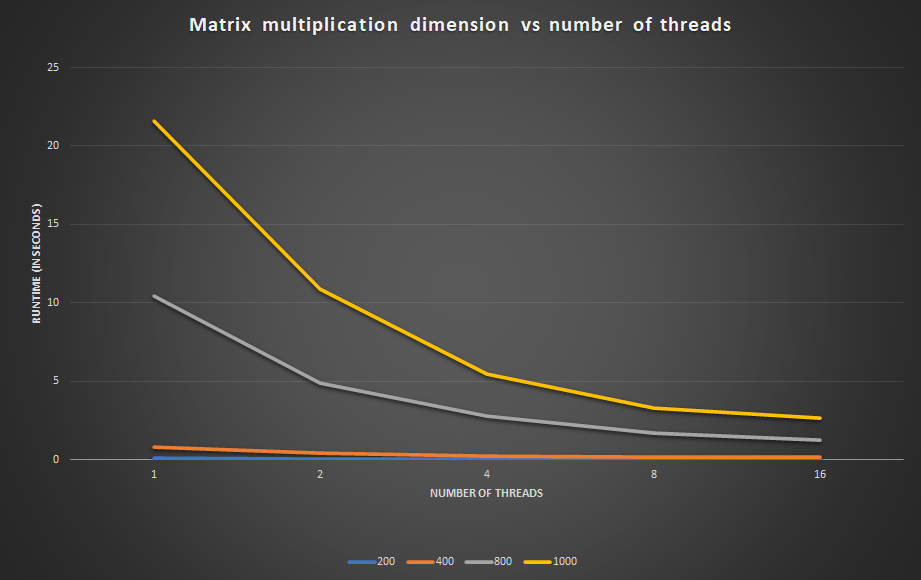
\includegraphics[width=\linewidth]{Figures/Matmul.png}
    \caption{
        Runtime of matrix multiplication with no of threads $t \in \{1,2,4,8,16\}$
        and dimensions $d \in \{200,400,800,1000\}$.
    }
    \label{fig:matmulspeedup}
\end{figure}

We tried to collapse the three for loops but we saw little improvement. We are
not sure exactly why this is. If only the outer loops is parallelised the threads
gets assigned a chunk of that loop which has two nested for loops inside. If We
collapse all three loops, the threads gets assigned a chunk of a single loop and
iterates through that and calculates values of $C$. According to our experiments,
both these cases is equally demanding for the threads and there is very little
difference. Since there was no difference, only the outer loop parallelisation
is plotted in figure \ref{fig:matmulspeedup}.

Many factors can explain this. One is that the work done at each iteration
is a simple sum that gets assigned and these are independent and a nested for
loop with as many iterations as a longer single for loop should take about the
same time. It is also unknown how the compiler handles this nested for loop and
if it vectorises it. What we know at least, is that empirically from our little experiment, collapsing
all loops does not improve the speed.
